\section{Marco teórico}

\noindent La metrología es la ciencia de las mediciones y sus aplicaciones
\parencite{jcgm_200_2012_vim}. La calibración relaciona la indicación de un
instrumento con el valor de un patrón de mayor exactitud y permite determinar el
error de indicación y su incertidumbre. La trazabilidad metrológica es la cadena
documentada de calibraciones que vincula el resultado con patrones nacionales o
internacionales. La incertidumbre de medición es el parámetro no negativo que
caracteriza la dispersión de los valores atribuibles al mensurando, evaluada con
componentes tipo~A y tipo~B conforme a la guía GUM~\parencite{jcgm2008gum}.

\subsection{Variables aleatorias discretas}
Para la deducción de las definiciones y ecuaciones de esta sección se seguirá
según~\cite{swendsen2012introduction} en el capítulo 3.

Un evento elemental es un resultado individual y exlusivo de un experimento, tal
que puede ocurrir una y solamente uno a la vez, Ejem. cuando se lanza una
moneda se tiene el resultado de que la moneda salga cara o sello.

\subsubsection{Variable aleatorias}
Sea $A = \set{a_j}_{j = 1}^N$ un conjunto de eventos elementales donde a cada
evento $a_j$ se le asigna una probabilidad $P(a_j)$, que por
simplicidad escribiremos (A, P(a)), a esto llamaremos
\textit{Variable aleatoria discreta}, si los eventos elementales son
números entonces a $(A, P(a))$ se le llama \textit{Número aleatorio}.
Por definicion de probablidad, para cada elemento se debe cumplir

\begin{equation}
  0 \leq P(a_j) \leq 1
  \label{eq:prob-elemental}
\end{equation}

Asi la probabilidad de todo el conjunto $A$ debe ser $1$, por lo que
debe, cumplirse
que

\begin{equation}
  \sum_{j = 1}^N P(a_j) = 1
  \label{eq:prob-total}
\end{equation}

Que por simplicidad escribiremos

\begin{equation}
  \sum_{a} P(a) = 1
  \label{eq:prob-total-sim}
\end{equation}

\subsubsection{Probablidad de multiples variables aleatorias discretas}
Supongamos que se tienen dos eventos elementales
$A=\set{a_i}_{i=1}^N$ y $B=\set{b_j}_{j=1}^M$,
entonces la probabilidad conjunta para $a_i$ y $b_j$ es

\begin{equation}
  0 \leq P(a_i, b_j) \leq 1
  \label{eq:prob-conjunta}
\end{equation}

y la probabilidad para todo el cunjunto de eventos elementales se debe cumplir

\begin{equation}
  \sum_{i=1}^N \sum_{j=1}^M P(a_i, b_j) = 1
  \label{eq:prob-conjunta-total}
\end{equation}

que por simplicidad escribiremos

\begin{equation}
  \sum_{a} \sum_{b} P(a, b) = 1
  \label{eq:prob-conjunta-total-sim}
\end{equation}

\paragraph*{Probabilidad marginal}
Si queremos recuperar la probablidad $P_A(a_j)$ al cual denominaremos
\textit{Probablidad marginal}, es lógico que sumaremos todas las
probablidades sobre $B$ así obtenemos

\begin{equation}
  P_A(a) = \sum_{b} P(a, b)
  \label{eq:prob-marginal}
\end{equation}

\paragraph*{Probabilidad condicional}
Supongamos que queremos la probablidad de que ocurra el evento
$a$ dado que ocurrio $b$ el cual notaremos como $P(a|b)$, asumiendo
que que la probablidad $P_B(b) \neq 0$ entonces esta será

\begin{equation}
  P(a|b) = \frac{P(a,b)}{P_B(b)}
  \label{eq:prob-condicional}
\end{equation}

% === Funciones aleatorias y Números Aleatorios ===
\subsubsection{Funciones aleatorias de una variable y Números Aleatorios}
Sea el conjunto de eventos elementales $A = \set{a_j}_{j = 1}^{N_A}$ junto a
su probablidad $P(a_i)$, podemos definir sobre este número aleatorio
una función númerica $F = \set{F(a_j)}_{j = 1}^{N_A}$ tal que

\begin{equation}
  P_F(f) = \sum_a \delta_{f,F(a)} P(a)
  \label{eq:f-prob}
\end{equation}

Donde $\delta_{f,F(a)}$ es la función \textit{Delta de Kroneker} de $f$ y $F(a)$

\begin{equation}
  \delta_{f,F(a)} =
  \begin{cases}
    1 & \text{si } f = F(a)\\
    0 & \text{si } f \neq F(a)
  \end{cases}
  \label{eq:delta-kron}
\end{equation}

el cual también será un número aleatorio.

Supongamos ahora que se tiene dos números aleatorios $X, Y$, con probablidad
$P(x, y)$ y se quiere una nueva función arbitraria $G(x, y)$, entonces
la distribución de probablidad de $G$ esta dado como una suma sobre
todas las combinaciónes de los eventeos $X$ y $Y$ con la delta de kronecker
tomando cada uno de los eventos particulares correspondientes a $G$

\begin{equation}
  P_G(g) = \sum_{x}\sum_y\delta_{g, G(x, y)} P(x, y)
  \label{eq:prob-g}
\end{equation}

\subsubsection{Media, Variancia y Desviación Estándar}

La media o promedio de una función $F(A)$, sobre $(A, P(a))$ se define
como

\begin{equation}
  \bk{F} = \sum_a F(a) P(a)
  \label{eq:d-mean}
\end{equation}

De manera similar el $n$-ésimo momento se define

\begin{equation}
  \bk{F^n} = \sum_a F^n(a) P(a)
  \label{eq:d-n-moment}
\end{equation}

Y el $n$-ésimo momento central

\begin{equation}
  \bk{(F - \bk{F})^n}
  = \sum_a (F^n(a) - \bk{F}^n)(a) P(a)
  \label{eq:d-central-moment}
\end{equation}

El segundo momento central se le denomina \textit{varianza}, $\sigma^2$ el cuál
será

\begin{align*}
  \sigma^2 &= \bk{(F - \bk{F})^2}\\
  &= \bk{F^2 - 2F\bk{F} + \bk{F}^2}\\
  &= \sum_a (F^2 - 2F\bk{F} + \bk{F}^2)(a) P(a)\\
  &= \sum_a F^2(a)P(a) - 2\bk{F}\sum_a F(a)P(a) + \bk{F}^2\sum_aP(a)\\
  &= \bk{F^2} - 2\bk{F}\bk{F} + \bk{F}^2
\end{align*}

\begin{equation}
  \therefore \sigma^2 = \bk{F^2} - \bk{F}^2
  \label{eq:d-var}
\end{equation}

Con esto podemos definir la desviación estándar como $\sigma = \sqrt{\sigma^2}$

\begin{equation}
  \sigma = \sqrt{\bk{F^2} - \bk{F}^2}
  \label{eq:d-std}
\end{equation}

\subsection{Funciones aleatorias Discretas de varias variables}

Sea $\mathcal A = \set{A_i}_{i=1}^M$ un conjunto de $M$ variables aleatorias
discretas, donde cada
$A_i = \set{a_{i1}, a_{i2}, \ldots, a_{iN_i}}$ es el conjunto de eventos
elementales o valores posibles de la $i$-ésima variable, con probabilidad
$P_{A_i}(a_{ij})$.

Ahora definamos el espacio muestral conjunto $\Omega$ como el producto
cartesiano de los espacios individuales
\begin{equation}
  \Omega := A_1 \times A_2 \times \cdots \times A_M
  = \set{\vec a = (a_1, a_2, \ldots, a_M) : a_i \in A_i}
  \label{eq:omega_total}
\end{equation}

Sobre este espacio se define la probabilidad conjunta
$P(\vec a) = P(a_1, \ldots, a_M)$, la cual debe cumplir las condiciones de no
negatividad y normalización
\begin{equation}
  P(\vec a) \ge 0 \quad \forall \vec a \in \Omega
  \quad \wedge \quad
  \sum_{\vec a \in \Omega} P(\vec a) = 1
  \label{eq:prob-normalization}
\end{equation}

Si consideramos un subconjunto de variables sobre el subespacio
$\Omega_j \subseteq \Omega$, la probabilidad marginal para una configuración
$\vec a \in \Omega_j$ se obtiene sumando la probabilidad conjunta sobre las
variables que no pertenecen a $\Omega_j$, esto es
\begin{equation}
  P_{\Omega_j}(\vec a)
  = \sum_{\vec a' \notin \Omega_j} P(\vec a, \vec a')
  \label{eq:prob-marginal-omega}
\end{equation}

Sobre este espacio se define un conjunto de funciones aleatorias
$F = \set{F_j}_{j=1}^N$, donde cada $F_j: \Omega_j \to \mathbb{R}$ es una
función escalar que asigna un valor real a cada evento $\vec a \in \Omega_j$.

Usando la Delta de Kronecker $\delta_{f, F_j(\vec a)}$, la distribución de
probabilidad $P_{F_j}(f)$, i.e. la probabilidad de que $F_j$ tome el valor
específico $f$, se expresa como
\begin{equation}
  P_{F_j}(f)
  = \sum_{\vec a \in \Omega_j} \delta_{f, F_j(\vec a)} \,
  P_{\Omega_j}(\vec a)
  \label{eq:prob-fj-kronecker}
\end{equation}

Con esta distribución, la media $\bk{F_j}$ está dada por
\begin{equation}
  \bk{F_j}
  = \sum_f f \, P_{F_j}(f)
  = \sum_f f \left(
    \sum_{\vec a \in \Omega_j} \delta_{f, F_j(\vec a)} \,
    P_{\Omega_j}(\vec a)
  \right)
  \label{eq:mean-fj-delta}
\end{equation}

\begin{equation}
  \sum_f f \, \delta_{f, F_j(\vec a)} = F_j(\vec a)
  \label{eq:kronecker-filtering}
\end{equation}

Intercambiando las sumas y usando la ecuación~\ref{eq:kronecker-filtering} se
recupera la definición usual de la media:
\begin{equation}
  \bk{F_j}
  = \sum_{\vec a \in \Omega_j} F_j(\vec a) \, P_{\Omega_j}(\vec a)
  \label{eq:mean:fj}
\end{equation}

Supongamos que se quiere una nueva variable aleatoria $S$:
\begin{equation}
  S(\vec a) = \sum_{j=1}^N F_j(\vec a), \quad \vec a \in \Omega
  \label{eq:s-set}
\end{equation}

Junto a la probabilidad $P(a_1, \ldots, a_M)$, entonces la media de $S$ está
dada por

\begin{align*}
  \bk S &= \bk{\sum_{j = 1}^N F_j}
  = \sum_{a_1}\cdots \sum_{a_M} \sum_{j = 1}^N F_j(\vec{a}) P(a_1,
  \ldots, a_M)\\
  &= \sum_{j = 1}^N \sum_{a_1} \cdots \sum_{a_M} F_j(\vec{a}) P(a_1,
  \ldots, a_M)
  = \sum_{j = 1}^N \sum_{\vec{a} \in \Omega_j} F_j(\vec{a} )
  \sum_{\vec{a} \not \in \Omega_j} P(a_1, \ldots, a_M) \\
\end{align*}

Pero las sumas sobre $\vec{a} \not \in \Omega_j$ dan la probabilidad marginal
$P_{\Omega_j}(\vec{a})$ por lo que

\begin{align*}
  \bk S = \sum_{j=1}^N \sum_{\vec a \in \Omega_j} F_j(\vec a)
  P_{\Omega_j}(\vec{a})
\end{align*}

Y esta última es la media de $F_j$ por lo que la media de $S$ es igual a
la suma de las medias

\begin{equation}
  \bk S = \bk{\sum_{j = 1}^N F_j} = \sum_{j = 1}^N \bk{F_j}
  \label{eq:mean-s}
\end{equation}

Si todas las funciones aleatorias $F_j$ tienen la misma media, i.e.
$\bk{F_j} = \bk{F}$, entonces

\begin{equation}
  \bk S = \sum_{ j = 1}^N \bk{F_j}= N \bk{F}
  \label{eq:mean-s-eq}
\end{equation}

\subsection{Varianza y Desviación Estándar de funciones aleatorias
de varias variables}

Ahora para calcular la varianza $\sigma^2_S$ de $S$ se puede utilizar
la definición

\begin{align*}
  \sigma^2_S &= \bk{S^2} - \bk{S}^2 = \bk{SS} - \bk{S}^2 = \bk{
  \sum_{j=1}^N F_j \sum_{k=1}^N F_k} - \sum_{j=1}^N \bk{F_j}
  \sum_{k=1}^N \bk{F_k}
  \\
  &= \bk{\sum_{j=1}^N \sum_{k=1}^N F_jF_k} - \sum_{j=1}^N \bk{F_j}
  \sum_{k=1}^N \bk{F_k}
\end{align*}

utilizando la ecuación~\ref{eq:mean-s} esta última
igualdad se convierte en

\begin{align}
  \sigma^2_S &= \sum_{j=1}^N \sum_{k=1}^N \bk{F_jF_k} - \sum_{j=1}^N
  \bk{F_j} \sum_{k=1}^N \bk{F_k}
\end{align}

Suponiendo que $F_j$ y $F_k$ son independientes por pares, podemos hacer

\begin{align*}
  \sigma^2_S &= \sum_{j=1}^N \sum_{k\neq j}^N \bk{F_j}\bk{F_k}
  + \sum_{j=1}^N \bk{F_j^2} - \sum_{j=1}^N \bk{F_j}\sum_{k\neq j}^N \bk{F_k}
  - \sum_{j=1}^N \bk{F_j}^2
  = \sum_{j=1}^N \left(
    \bk{F_j^2} - \bk{F_j}^2
  \right)
\end{align*}

Por lo tanto tenemos que

\begin{equation}
  \sigma^2_S = \sum_{j=1}^N \sigma^2_j
  \label{eq:var-s}
\end{equation}

Con lo que podemos obtener la desviación estándar $\sigma_S$ como

\begin{equation}
  \sigma_S = \sqrt{\sigma^2_S}
  \label{eq:std-s}
\end{equation}

De la misma forma, si todas las funciones aleatorias $F_j$ tienen la misma
varianza, i.e. $\sigma^2_j = \sigma^2$, entonces

\begin{equation}
  \sigma^2_S = \sum_{j=1}^N \sigma^2_j = N \sigma^2
  \label{eq:var-s-eq}
\end{equation}

Y por lo tanto

\begin{equation}
  \sigma_S = \sigma\sqrt{N}
  \label{eq:std-s-eq}
\end{equation}

Y por lo tanto la desviación estándar relativa decrece con la raíz
cuadrada del número de variables.

\begin{equation}
  \frac{\sigma_S}{\bk{S}} = \frac{\sigma\sqrt{N}}{N\bk{F}}
  = \frac{\sigma}{\sqrt{N}\bk{F}}
  \label{eq:std-relative}
\end{equation}

\subsubsection{Varianza de una muestra y el factor
\texorpdfstring{$1/(n-1)$}{1/(n-1)}}

En las secciones previas se definió el valor medio teorico como $\mu
= \langle x \rangle$. Pero en un experimento solo tenemos $n$
mediciones independientes $\{x_1, \dots, x_n\}$, asi que usamos el promedio:

\begin{equation}
  \bk{x}_n = \frac{1}{n} \sum_{i=1}^n x_i
  \label{eq:media-muestral}
\end{equation}

Si usamos el promedio $\bk{x}_n$ en vez del valor medio $\mu$, estamos
subestimando la dispersion. Para ver esto escribimos la desviacion de
cada medicion sumando y restando $\mu$:

\begin{equation}
  x_i - \bk{x}_n = (x_i - \mu) - (\bk{x}_n - \mu)
\end{equation}

Elevando al cuadrado y sumando sobre las $n$ mediciones:

\begin{align}
  \sum_{i=1}^n (x_i - \bk{x}_n)^2 &= \sum_{i=1}^n \left[ (x_i - \mu) -
  (\bk{x}_n - \mu) \right]^2 \nonumber \\
  &= \sum_{i=1}^n (x_i - \mu)^2 - 2(\bk{x}_n - \mu) \sum_{i=1}^n (x_i
  - \mu) + \sum_{i=1}^n (\bk{x}_n - \mu)^2
\end{align}

Puesto que $\sum_{i=1}^n (x_i - \mu) = n(\bk{x}_n - \mu)$, la suma se reduce a:

\begin{equation}
  \sum_{i=1}^n (x_i - \bk{x}_n)^2 = \sum_{i=1}^n (x_i - \mu)^2 -
  n(\bk{x}_n - \mu)^2
  \label{eq:descomposicion-residuos}
\end{equation}

Ahora aplicamos el valor esperado $\langle \cdots \rangle$:

\begin{equation}
  \left\langle \sum_{i=1}^n (x_i - \bk{x}_n)^2 \right\rangle =
  \sum_{i=1}^n \langle (x_i - \mu)^2 \rangle - n \langle (\bk{x}_n -
  \mu)^2 \rangle
  \label{eq:esperanza-residuos}
\end{equation}

Recordando que por definicion de varianza (ecuación~\eqref{eq:d-var})
$\langle (x_i - \mu)^2 \rangle = \sigma^2$, y que la varianza del
promedio (ecuación~\eqref{eq:std-relative}) cumple $\langle (\bk{x}_n
- \mu)^2 \rangle = \sigma^2 / n$, entonces:

\begin{align}
  \left\langle \sum_{i=1}^n (x_i - \bk{x}_n)^2 \right\rangle &=
  n\sigma^2 - n\left(\frac{\sigma^2}{n}\right) \nonumber \\
  &= (n - 1)\sigma^2
  \label{eq:esperanza-bessel}
\end{align}

Por lo tanto, para que nuestra estimacion coincida con la varianza
$\sigma^2$ (o sea $\langle s^2 \rangle = \sigma^2$), tenemos que
dividir entre $n - 1$:

\begin{equation}
  s^2 = \frac{1}{n - 1} \sum_{i=1}^n (x_i - \bk{x}_n)^2
  \label{eq:varianza-muestral-insesgada}
\end{equation}

Con lo cual la desviacion estandar del promedio queda:

\begin{equation}
  \sigma(\bk{x}_n) = \frac{s}{\sqrt{n}}
  \label{eq:sigma-media-experimental}
\end{equation}

La desviación estándar de la media de la
ecuación~\eqref{eq:sigma-media-experimental} proviene de observaciones
repetidas y constituye lo que la GUM~\parencite{jcgm2008gum} denomina
\textit{evaluación tipo~A} de la incertidumbre.

No todas las componentes se estiman así. Cuando la información disponible
no proviene de repeticiones sino de una especificación del fabricante, un
certificado de calibración o una frontera acotada conocida, la GUM
denomina a su tratamiento \textit{evaluación tipo~B}. En ese caso no se
aplica la ecuación~\eqref{eq:sigma-media-experimental}, sino que la
dispersión se deduce de la distribución de probabilidad que describe la
información disponible. El caso más frecuente es la distribución
rectangular, que se desarrolla a continuación.

\subsubsection{Funciones aleatorias continuas}
Utilizando la misma lógica de las secciones anteriores, se puede
hacer las siguientes definiciones para funciones aleatorias continuas.

Sea $P(\vec{a}) \geq 0$ una función de probabilidad de densidad
$\vec{a} \in \Omega = \set{(a_{1}, a_{2}, \ldots, a_{N}): a_i \in
\mathbb{R} }$, y denotaremos como $d^N a$ al diferencial sobre $\Omega$,
por lo que la probabilidad sobre $\Omega$ debe cumplir

\begin{gather}
  \int\dots\int_{\Omega}  P(\vec{a})\, da_1 \cdots d a_N = 1
  \label{eq:prob-aleatoria-continua}
\end{gather}

donde en vez de usar esta notación, usaremos la forma corta.

\begin{equation}
  \int_\Omega P(\vec{a})\,d^Na
  \label{eq:eq-prob-random-continue}
\end{equation}

Ahora definamos una función aleatoria continua $F: \Omega \to \mathbb{R}$
por lo que la media de $F$ será

\begin{equation}
  \bk{F} = \int_\Omega F(\vec{a}) P(\vec{a})\, d^Na
  \label{eq:mean-con-mult}
\end{equation}

El $n$-esimo momento de $F$ será

\begin{equation}
  \bk{F^n} = \int_\Omega F^n(\vec{a}) P(\vec{a}) d^N\vec{a}
  \label{eq:moment-con-mult}
\end{equation}

El $n$-simo momento central de $F$ será

\begin{equation}
  \bk{(F - \bk{F})^n}
  \label{eq:n-central-moment-con-mult}
\end{equation}

Y la desviación estandar de $F$ será

\begin{equation}
  \sigma^2 = \bk{(F - \bk{F})^2} = \bk{F^2} - \bk{F}^2
  \label{eq:std-con-mult}
\end{equation}

\paragraph{Distribución continua uniforme (rectangular)}

Supongamos una variable aleatoria continua $x$ acotada dentro de un intervalo simétrico $[-a, a]$ de amplitud total $\Delta = 2a$. En ausencia de información adicional que privilegie algún punto del intervalo, asignamos una densidad de probabilidad uniforme constante $P(x) = C$.

Por la condición de normalización de la ecuación~\eqref{eq:prob-aleatoria-continua}:

\begin{equation}
    \int_{-a}^{a} P(x) \, dx = C \int_{-a}^{a} dx = C(2a) = 1
    \quad\Longrightarrow\quad
    C = \frac{1}{2a}
\end{equation}

por lo que la función de densidad queda:

\begin{equation}
    P(x) =
    \begin{cases}
        \dfrac{1}{2a}, & x \in [-a, a] \\[6pt]
        0, & x \notin [-a, a]
    \end{cases}
    \label{eq:distribucion-rectangular}
\end{equation}

Puesto que $P(x)$ es una función par respecto al origen, el valor medio es nulo:

\begin{equation}
    \langle x \rangle = \int_{-a}^{a} x P(x) \, dx = \frac{1}{2a} \int_{-a}^{a} x \, dx = 0
\end{equation}

Evaluando la varianza mediante el segundo momento central de la ecuación~\eqref{eq:std-con-mult}:

\begin{equation}
    \sigma^2 = \langle x^2 \rangle - \langle x \rangle^2
    = \int_{-a}^{a} x^2 P(x) \, dx
    = \frac{1}{2a} \left[ \frac{x^3}{3} \right]_{-a}^{a}
    = \frac{a^2}{3}
\end{equation}

Extrayendo la raíz cuadrada, la desviación estándar de la distribución rectangular resulta:

\begin{equation}
    \sigma = \frac{a}{\sqrt{3}} = \frac{\Delta}{2\sqrt{3}}
    \label{eq:sigma-rectangular}
\end{equation}

donde $a$ es la semiamplitud del intervalo y $\Delta = 2a$ su ancho total.

\paragraph{Distribuciones triangular y normal}

En una evaluación tipo~B la distribución se elige según la información
disponible. Si los valores son más probables cerca del centro del intervalo, se
usa la distribución triangular,

\begin{equation}
    \sigma = \frac{a}{\sqrt{6}}.
    \label{eq:sigma-triangular}
\end{equation}

Si la componente proviene de un certificado que declara una incertidumbre
expandida $U$ con factor de cobertura $k$, se usa la distribución normal,

\begin{equation}
    \sigma = \frac{U}{k},
    \label{eq:sigma-normal}
\end{equation}

con $k=2$ para un nivel de confianza aproximado del $95$\,\%
\parencite{jcgm2008gum}.

De manera análoga a la función delta de Kroneker se define
la función delta $\delta_\epsilon(x)$ como sigue

\begin{equation}
  \delta_\epsilon (x) =
  \begin{cases}
    0 & \text{si } x < \epsilon\\
    \frac{1}{2\epsilon} & \text{si } -\epsilon \leq x \leq \epsilon\\
    0 & \text{si } x > \epsilon
  \end{cases}
  \label{eq:delta}
\end{equation}

Por lo que la integral sobre $[-\epsilon, \epsilon] \subset
\Omega \subset \mathbb R$ será

\begin{equation}
  \int_{-\infty}^\infty \delta_\epsilon(cx - d)\, dx = \int_\Omega
  \delta_\epsilon(cx - d) dx = \frac{1}{|c|}
  \label{eq:delta-integral}
\end{equation}

Con esto la función \textit{Delta de Dirac} se puede definir como

\begin{equation}
  \delta(x) = \lim_{\epsilon \to 0} \delta_\epsilon(x)
  \label{eq:delta-dirac}
\end{equation}

y así la integral de $f(x)\delta(c(x - x_0))$ sobre $\Omega$ será

\begin{equation}
  \int_{-\infty}^\infty f(x)\delta(c(x - x_0))\,dx = \frac{f(x_0)}{|c|}
  \label{eq:dalta-dirac-integral}
\end{equation}

Asi tomando una función análitica sobre una región $x_0 \in \Omega$, y
una función $g(x)$ análitica y derivable con ceros en
$\left\{x_j\right\}_{j=1}^N$ y $g'(x_j) \neq 0 $, resulta que

\begin{equation}
  \int_{-\infty}^\infty f(x)\delta(g(x))\,dx = \sum_{j=1}^N
  \frac{f(x_j)}{|g'(x_j)|}
  \label{eq:delta-dirac-integral-2}
\end{equation}

suponiengo que se tiene dos variables aleatorias, $x$ y $y$,
junto a su densidad de probablidad, $P(x, y)$, y se define una
nueva variable aleatoria, $s$, la cual es alguna
función sobre las variables aleatorias originales, $x$ y $y$,
$s = f(x, y)$. Entonces la nueva funsión de densidad
$P(s)$ puede ser escrita como:

\begin{equation}
  P(s) = \int_{-\infty}^{\infty}\int_{-\infty}^{\infty} P(x, y)
  \delta(s - f(x, y))\, dx dy
  \label{eq:new-con-pdf}
\end{equation}

Por lo que integrando sobre $\Omega$ se obtiene la normalización

\begin{align*}
  \int_{-\infty}^{\infty} P(s)\, ds &=
  \int_{-\infty}^{\infty}\int_{-\infty}^{\infty}
  \int_{-\infty}^{\infty} P(x, y) \delta(s - f(x, y))\, dx dy ds\\
  &= \int_{-\infty}^{\infty} \int_{-\infty}^{\infty} P(x, y)\, dx dy = 1
  \label{eq:normalizacion-con-mult}
\end{align*}

\subsection{Propagación de error}
\label{sec:propagacion}
Sea $F: \mathbb R^N \to \mathbb R$ una función continua cuya
regla de correspondencia es $F = F(\vec{x})$
tal que $\vec{x} = (x_1, \cdots, x_N) \in \mathbb R^N$ donde $x_j$ es
una variable
aleatoria continua, estas variables pueden estar asociadas
a cualquier medición física experimental la cual tienen
una de densidad de probabilidad conjunta $P(x)$. $F(\vec{x})$
Puede ser expresado como la suma de su valor medio $\bk{F}$
y una variación aleatoria o error $E(\vec{x})$:

\begin{equation}
  F(x) = \bk{F} + E(x) \implies E(x) = F(x) - \bk{F}
  \label{eq:error-func}
\end{equation}

Calculando el valor medio de $E(x)$

\begin{align*}
  \bk{E} &= \bk{F - \bk{F}}\\
  &= \int_\Omega \left(F(\vec{x}) - \bk{F}\right)P(\vec{x})d^Nx\\
  &= \int_\Omega F(\vec{x})P(\vec{x})d^Nx
  - \bk F\int_\Omega P(\vec{x})d^Nx\\
  &=\bk F - \bk F \\
  \therefore \bk{E} &= 0
\end{align*}

Ahora calculemos la varianza de $F$ en función de $E$,
por lo que tendremos

\begin{equation}
  \sigma_E^2 = \bk{E^2} - \bk E^2 = \bk{E^2} = \int_\Omega
  E^2(\vec{x}) P(\vec{x}) d^Nx
  \label{eq:medition-variance}
\end{equation}

Pero necesitamos la regla de correspondencia de $E(\vec{x})$.
Tomemos la ecuación~\ref{eq:error-func} la cual
podemos aproximar por series de Taylor, para eso tomemos el valor
medio $\mu_i = \bk{x_i}$,
con estos valores tomemos el vector medio $\vec{\mu} = (\mu_1, \dots, \mu_N)$,
por lo que si aproximamos a $F$ al rededor de $F(\vec{u})$

\begin{equation}
  F(x) = F(\vec\mu) + \sum_{i = 1}^N \pti{F} (x_i - \mu_i) +
  \mathcal{O}((\vec{x}-\mu)^2)
  \label{eq:taylor-f-aprox}
\end{equation}

Descartando los términos cuadráticos $\mathcal{O}(\vec{x}-\vec\mu)^2$
por que se vuelven demasiado pequeños podemos calcular su valor medio

\begin{equation}
  \bk{F} \approx \bk{F(\vec\mu) + \sum_{i = 1}^N \pti{F} (x_i - \mu_i)}
  = \bk{F(\vec\mu)} + \bk{\sum_{i = 1}^N \pti{F} (x_i - \mu_i)}
  \label{eq:F-mean-value}
\end{equation}

se puede observar que $\bk{F(\mu)} = F(\mu)$ ademas identificando el segundo
termino del lado derecho como $\bk{E(x)}$, Puesto qué

\begin{equation*}
  \bk{\sum_{i = 1}^N \pti{F} (x_i - \mu_i)}
  = \sum_{i = 1}^N \pti{F} \int_\Omega (x_i - \mu_i)P(\vec x)\, d^N x
  = \sum_{i = 1}^N \pti{F} (\underbrace{\bk {x_i}}_{\mu_i} - \mu_i)
  = 0
\end{equation*}

La cuál es una ecuación aproximada de la ecuación (\ref{eq:error-func})

\begin{equation}
  \bk{F} \approx F(\mu)\quad \wedge \quad E(x) = \sum_{i = 1}^N
  \pti{F} (x_i - \mu_i)
  \label{eq:F-mean}
\end{equation}

Reemplazando $E(x)$ en la ecuación (\ref{eq:medition-variance})
\begin{align*}
  \sigma_F^2 &= \int_\Omega \left(
    \sum_{i = 1}^N \pti{F} (x_i - \mu_i)
  \right)^2 P(\vec x)\, d^Nx\\
  &= \int_\Omega
  \left(
    \sum_{i = 1}^N \pti{F} (x_i - \mu_i)
  \right)
  \left(
    \sum_{j = 1}^N \pti{F} (x_j - \mu_j)
  \right)P(\vec x)\,d^Nx\\
  &=\sum_{i=1}^N\left(\pti{F}\right)^2
  \underbrace{\int_\Omega(x_i-u_i)^2d^Nx}_{\sigma^2_{x_i}}\\
  &\qquad\qquad+\sum_{i=1}^N \sum_{j\neq i}^N\pti{F}\ptj{F}
  \underbrace{
    \int_\Omega(x_i -\mu_i)(x_j - \mu_j)P(\vec x)\, d^Nx
  }_{\text{Cov}(x_i, x_j)}
\end{align*}

Si consideremos a $x_i$ y $y_i$ independientes
(como podría ser medición de la longitud y temperatura), entonces
${\text{Cov}(x_i, x_j)} = 0$, pues

\begin{align*}
  \text{Cov}(x_i, x_j) &= \int_\Omega (x_i - \mu_i)(x_j - \mu_j)
  P(\vec x) d^Nx \\
  &= \left(\int_\Omega (x_i - \mu_i)P(\vec x) d^Nx\right)
  \left(\int_\Omega (x_j - \mu_j)P(\vec x) d^Nx\right)\\
  &= \left(\underbrace{\bk {x_i}}_{\mu_i} - \mu_j\right)
  \left(\underbrace{\bk {x_j}}_{\mu_j} - \mu_j\right)\\
  \\
  \therefore \text{Cov}(x_i, x_j) &= 0
\end{align*}

Con lo que finalmente para $F(x) = \bk F + E(x)$ podemos escribir como

\begin{equation}
  F(x) \approx \bk F \pm \sigma_F
  \label{eq:error-std}
\end{equation}

Donde

\begin{equation}
  \bk F = F(\mu) \qquad \wedge \qquad \sigma_F =
  \sqrt{\sum_{i=1}^N\left(\pti{F}\right)^2\sigma^2_{x_i}}
  \label{eq:error-std-values}
\end{equation}

Para el caso discreto $\sigma^2_{x_i}$ se puede calcular como
\begin{equation}
  \sigma^2_{x_i} = \sum_x (x_i - \mu_i)^2 P(x)
  \label{eq:discrete-std-x-i}
\end{equation}


\subsubsection{Simbología y correspondencia con las normas}
\label{sec:simbologia}

La Tabla~\ref{tab:simbologia} recoge los símbolos empleados en el informe y su
equivalencia con la notación de la GUM y de los procedimientos de calibración del
INACAL. En 3.1, $\sigma$ denota la desviación estándar poblacional de una variable
aleatoria; en las secciones de calibración, $u$ denota la incertidumbre estándar.

\begin{table}[H]
\centering
\small
\renewcommand{\arraystretch}{1.15}
\caption{Simbología del informe y correspondencia con la GUM y el INACAL.}
\label{tab:simbologia}
\begin{tabular}{@{}p{2.5cm}p{7.3cm}p{1.3cm}p{4.1cm}@{}}
\toprule
Símbolo & Significado & Unidad & Equivalencia \\
\midrule
\multicolumn{4}{l}{\textit{Estadística}} \\
$x_i$ & observación individual & --- & --- \\
$\bar{x}$ & media muestral & --- & GUM 4.2 \\
$s$ & desviación estándar experimental & --- & GUM 4.2 \\
$s/\sqrt{n}$ & incertidumbre de la media & --- & $u_A$ (GUM 4.2) \\
$n$ & número de observaciones & --- & --- \\
$\sigma$ & desviación estándar poblacional & --- & --- \\
$a$ & semiamplitud de un intervalo & --- & GUM 4.3 \\
\midrule
\multicolumn{4}{l}{\textit{Incertidumbre}} \\
$u$ & incertidumbre estándar & --- & GUM 2.3 \\
$u_A$ & componente tipo~A & --- & GUM 4.2 \\
$u_B$ & componente tipo~B & --- & GUM 4.3 \\
$u_c$ & incertidumbre estándar combinada & --- & GUM 5 \\
$U$ & incertidumbre expandida & --- & GUM 6 \\
$k$ & factor de cobertura & --- & GUM 6 \\
\midrule
\multicolumn{4}{l}{\textit{Calibración dimensional}} \\
$I$, $I_k$ & indicación del instrumento & mm & $L_i$ (PC-012, PC-014) \\
$L_i$ & indicación del instrumento en la notación PC-012 & mm & equivale a $I$ \\
$X_j$ & lectura en la posición $j$ (superior, central, inferior) & mm & PC-012 \\
$D_j$ & diferencia entre la lectura $j$ y el valor patrón corregido & µm & PC-012 \\
$PC$ & promedio corregido de las lecturas & mm & PC-012 \\
$S_{E-I}$, $S_{E-P}$ & error por cambio de escala exteriores-interiores y exteriores-profundidad & µm & PC-012 \\
$VP$ & valor patrón & mm & PC-012, PC-014 \\
$VPC$ & valor patrón corregido & mm & PC-012 \\
$E$ & error de indicación & µm & PC-012, PC-014 \\
$E_{corr}$ & error de indicación corregido & µm & PC-012, PC-014 \\
$f_e$ & alcance del error de indicación & µm & PC-012 \\
$R$ & rango de repeticiones & µm & PC-012 \\
$f_w$ & alcance de repetibilidad & µm & PC-012 \\
$s_R$ & desviación estándar de las repeticiones & µm & GUM 4.2 \\
$d$ & división de escala & mm & PC-012 \\
$m$ & subdivisiones de la escala & --- & PC-012 \\
$r = d/m$ & resolución & mm & PC-012 \\
$L_{BP}$ & longitud del bloque patrón & mm & PC-014 \\
$U_{cal}$ & incertidumbre del certificado & µm & GUM 4.3 \\
$U_{der}$ & deriva del patrón & µm & ISO 3650 \\
$\alpha$ & coeficiente de dilatación & °C$^{-1}$ & PC-012, PC-014 \\
$\Delta T$ & desviación de temperatura & °C & PC-012, PC-014 \\
$t_\parallel$ & tolerancia de planitud & µm & PC-014 \\
\midrule
\multicolumn{4}{l}{\textit{Ultrasonido}} \\
$e$ & espesor medido & mm & PC-029 \\
$c_L$ & velocidad longitudinal & m/s & PC-029 \\
$\Delta t$ & tiempo de vuelo & s & PC-029 \\
$V_{PE}$ & valor del patrón escalonado & mm & PC-029 \\
$r$ & resolución del display & mm & PC-029 \\
\bottomrule
\end{tabular}
\end{table}


\subsection{Instrumentos de medición}
\label{sec:instrumentos}

Los equipos empleados se enumeran a continuación; los procedimientos y resultados
de calibración se presentan en la Sección~\ref{sec:procedimientos}.

\subsubsection{Instrumentos de medición dimensional y metrología industrial}
\label{sec:instr-dimensional}

\paragraph{Pie de rey o calibrador vernier}
\label{sec:instr-pie-de-rey}

El pie de rey es un instrumento de medición directa que determina dimensiones
lineales exteriores, interiores y de profundidad. Consta de una regla principal
graduada en milímetros y de un cursor móvil provisto de una escala secundaria o
nonio, que subdivide la menor división de la escala principal y aumenta la
resolución de lectura. El calibrador Mitutoyo Serie 530, código
\mbox{530-115} y número de serie 2013G454, tiene un alcance de $0$ a
$300\ \text{mm}$ y una división de escala de $d = 0{,}05\ \text{mm}$, derivada de
$20$ divisiones del nonio \parencite{mitutoyo_530_115}. La resolución se deduce
de la geometría de la escala en la Sección~\ref{sec:pie-de-rey}. El instrumento
dispone de mordazas rectificadas para medidas exteriores, orejetas superiores
para diámetros interiores y una varilla posterior deslizante para cavidades
profundas. Su calibración se efectuó por comparación directa con bloques patrón
según el procedimiento PC-012 del SNM-INDECOPI \parencite{inacal_pc012}.

\begin{figure}[H]
  \centering
  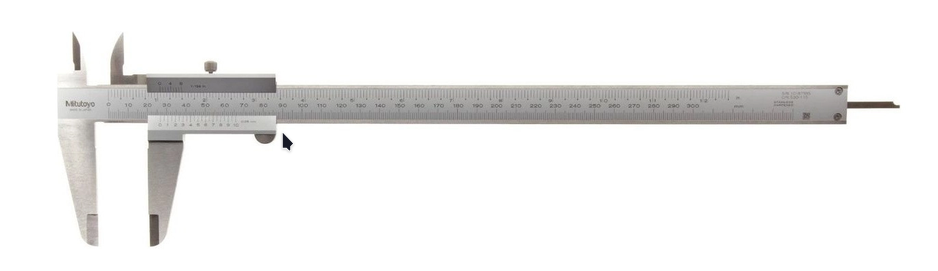
\includegraphics[width=0.55\textwidth]{img/bernier_pie_de_rey.png}
  \caption{Pie de rey Mitutoyo Serie 530, código 530-115.}
  \label{fig:pie-de-rey-instrumento}
\end{figure}

\paragraph{Medidor de profundidad digital}
\label{sec:instr-profundidad}

El medidor de profundidad digital determina la dimensión axial interna de
cavidades, ranuras, escalones y agujeros. Una base plana de apoyo se asienta
sobre la superficie de referencia y un vástago móvil se desplaza
perpendicularmente hasta el fondo del elemento inspeccionado. El medidor INSIZE
de la Serie 1147 tiene resolución de $0{,}01\ \text{mm}$
($0{,}0005''$) y pantalla LCD de lectura directa en milímetros o pulgadas
\parencite{insize_1147_depth}. El equipo dispone de puesta a cero (\texttt{ZERO})
en cualquier posición del recorrido y de conmutación de unidades
(\texttt{mm/inch}), lo que reduce los errores de alineación angular y facilita
la lectura. A diferencia del pie de rey, la base de apoyo no depende de la
posición de las mordazas, por lo que resulta adecuado para cavidades de acceso
restringido.

\begin{figure}[H]
  \centering
  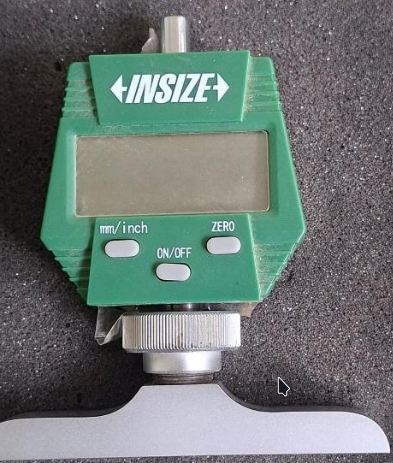
\includegraphics[width=0.30\textwidth]{img/profundidad.png}
  \caption{Medidor de profundidad digital INSIZE Serie 1147, con base de apoyo
  y controles \texttt{ZERO} y \texttt{mm/inch}.}
  \label{fig:profundidad-instrumento}
\end{figure}

\paragraph{Reloj comparador digital}
\label{sec:instr-reloj}

El comparador mide pequeñas desviaciones dimensionales y de forma por
comparación: transforma el desplazamiento axial del palpador en una indicación
de alta resolución. El comparador digital Mitutoyo ID-S1012M, código
\mbox{543-682/543-682B} y número de serie 12038057, tiene un alcance de
$0$ a $12{,}7\ \text{mm}$, una resolución de $0{,}01\ \text{mm}$ y una
exactitud de $\pm 0{,}02\ \text{mm}$ \parencite{mitutoyo_ids1012m}. Se usa en la
verificación de excentricidades, paralelismos y planitudes sobre una mesa de
granito. ISO~463:2006 define la terminología y las características metrológicas
de los comparadores mecánicos de cuadrante; se cita solo como referencia de los
errores de indicación \parencite{iso463_2006}. La calibración se realizó por
comparación con bloques patrón según el procedimiento PC-014 del
INACAL~\parencite{inacal_pc014}, desarrollada en la
Sección~\ref{sec:reloj-comparador}.

\begin{figure}[H]
  \centering
  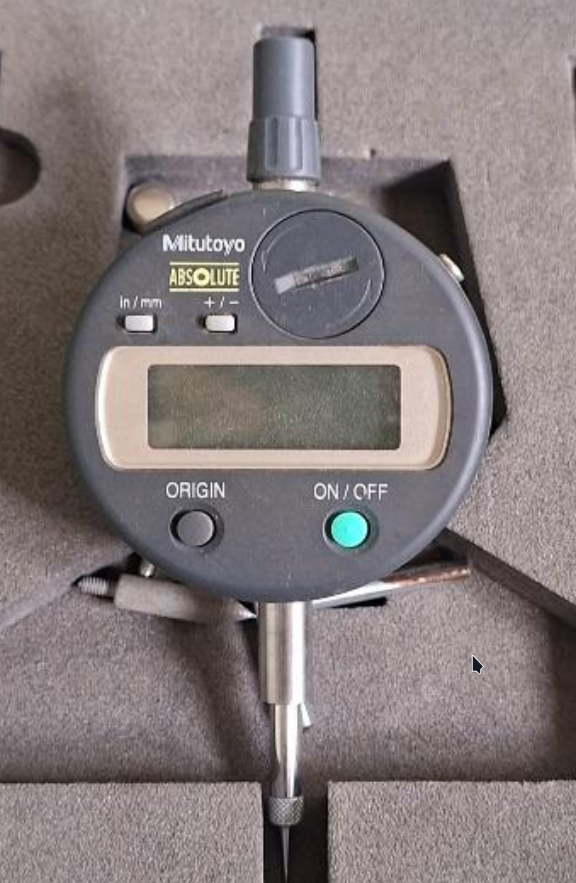
\includegraphics[width=0.30\textwidth]{img/comparator_clock.png}
  \caption{Detalle del comparador digital Mitutoyo ABSOLUTE utilizado en la
  calibración.}
  \label{fig:reloj-instrumento}
\end{figure}

\subsubsection{Equipos y patrones de ultrasonido y acústica}
\label{sec:instr-ut}

\paragraph{Medidor de espesores por ultrasonido}
\label{sec:instr-medidor-ut}

El medidor de espesores por ultrasonido es un equipo de ensayos no destructivos
que determina el grosor de una pared desde un solo acceso, sin alterar la
estructura evaluada. Funciona por el método de eco de pulso: un transductor
emite un impulso ultrasónico que se refleja en la cara posterior y el equipo
mide el tiempo de vuelo $\Delta t$ para calcular $d = c_L\,\Delta t/2$,
relación deducida en la Sección~\ref{sec:ut}
(ecuación~\eqref{eq:espesor-tof}). El medidor INSIZE ISU-100D lleva un
transductor piezoeléctrico de contacto de $5\ \text{MHz}$, un rango de $0{,}8$ a
$300\ \text{mm}$ y una resolución de $0{,}01\ \text{mm}$ \parencite{insize_isu100d}.
Para evitar la atenuación de la onda en la interfaz sonda--pieza se aplica gel
de glicerina como acoplante acústico. La calibración y la verificación de
linealidad se realizaron según el procedimiento PC-029 del
INACAL~\parencite{inacal_pc029} y la práctica ASTM E797~\parencite{astm_e797},
con los resultados recogidos en la Sección~\ref{sec:ut-calibracion}.

\begin{figure}[H]
  \centering
  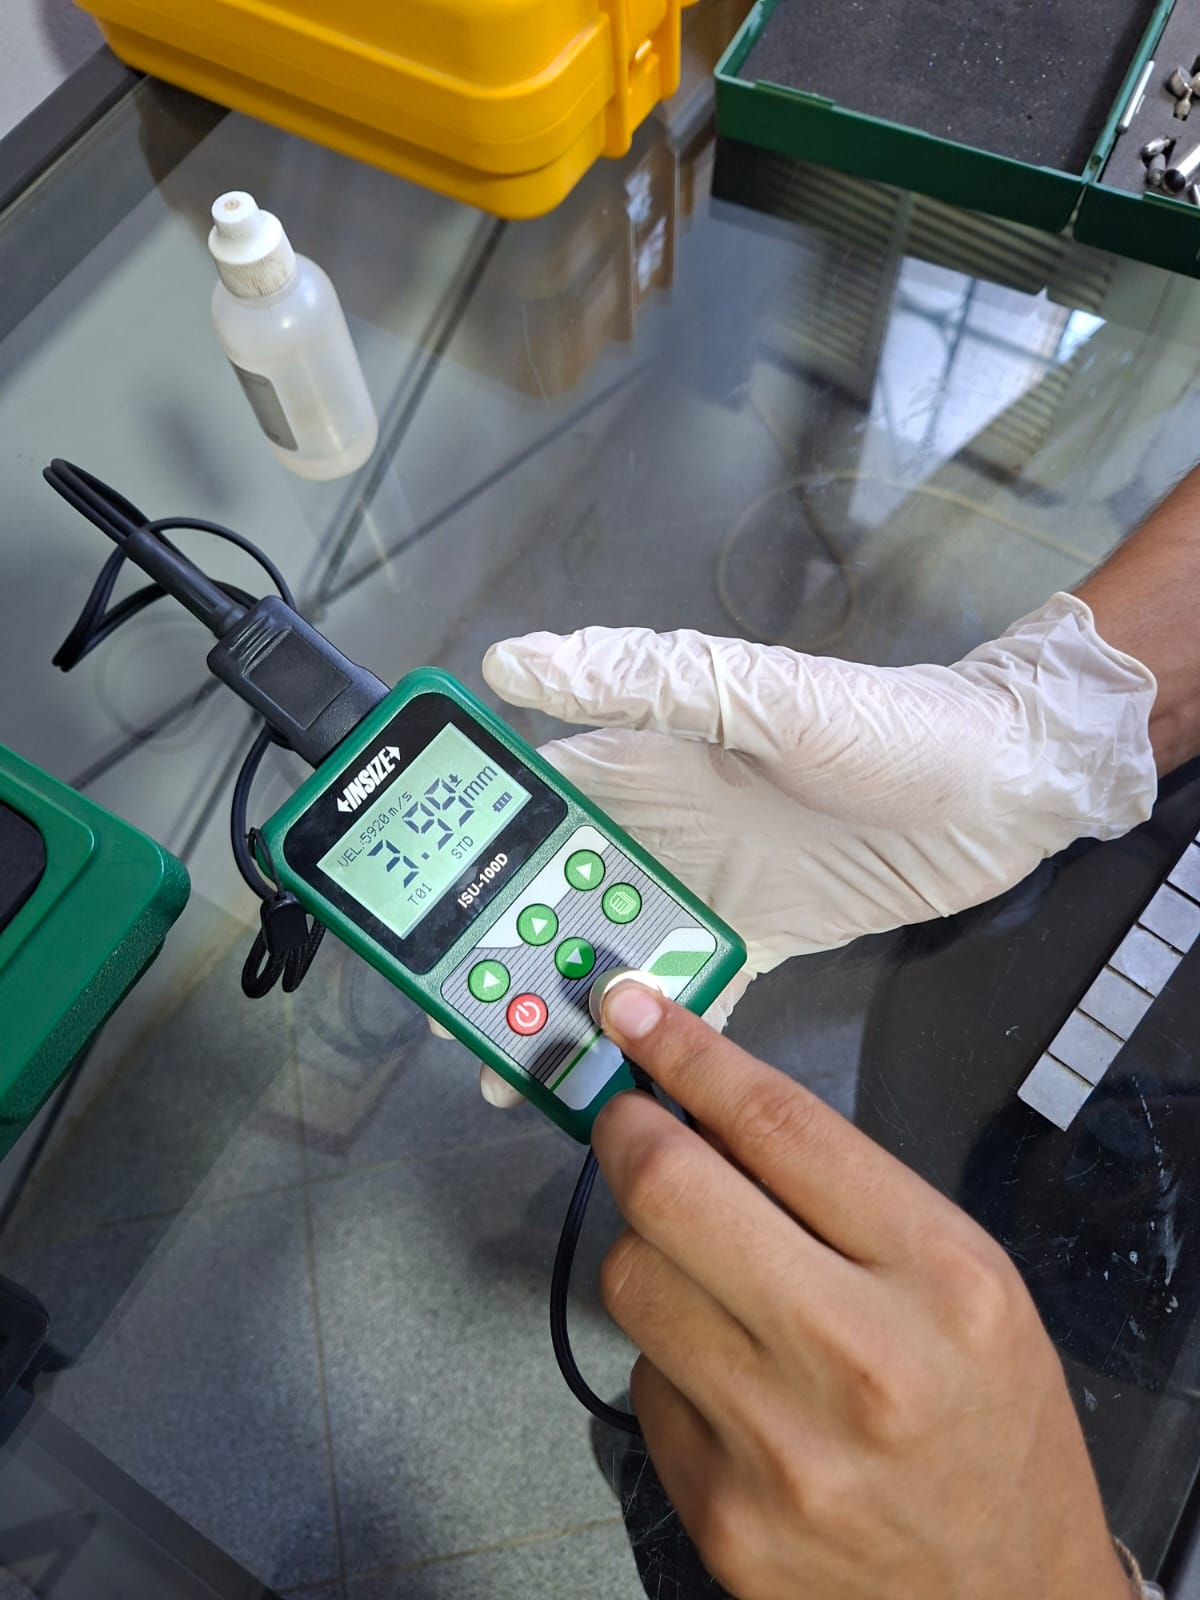
\includegraphics[width=0.42\textwidth]{img/ultrasound_instrument.jpeg}
  \caption{Medidor INSIZE ISU-100D con el transductor de 5 MHz y el acoplante.}
  \label{fig:ut-instrumento}
\end{figure}

\paragraph{Bloque patrón escalonado de espesores}
\label{sec:instr-step-block}

El bloque escalonado es un patrón de referencia empleado para ajustar la
velocidad del sonido, verificar la linealidad de escala y calibrar medidores de
espesores por ultrasonido. Consiste en un bloque de acero con diez niveles de
espesor conocido, de $2{,}50$ a $25{,}00\ \text{mm}$ en pasos de $2{,}50\ \text{mm}$.
Cada escalón permite comprobar la respuesta del transductor en un punto del
rango operativo, de modo que las mediciones de espesor quedan trazadas al patrón
certificado. Su empleo se rige por el procedimiento PC-029 \parencite{inacal_pc029}.

\begin{figure}[H]
  \centering
  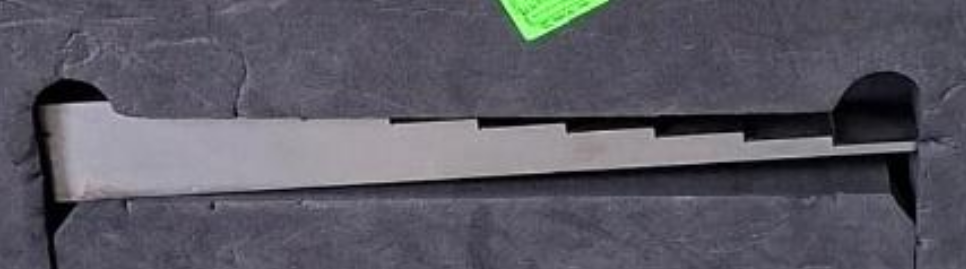
\includegraphics[width=0.55\textwidth]{img/scalonated_block.png}
  \caption{Bloque patrón escalonado de acero, de $2{,}50$ a $25{,}00\ \text{mm}$.}
  \label{fig:step-block-instrumento}
\end{figure}

\subsubsection{Patrones físicos de referencia y trazabilidad metrológica}
\label{sec:instr-bloques}

\paragraph{Bloques patrón de longitud certificados}

Los bloques patrón son estándares prismáticos de longitud, fabricados en acero
de alta estabilidad dimensional, cuyas caras opuestas presentan un pulido plano
de calidad lapidada. Materializan magnitudes fijas con incertidumbres
certificadas y garantizan la cadena de trazabilidad al metro del Sistema
Internacional de Unidades. ISO~3650:1998 especifica sus características
metrológicas y define los grados de exactitud K, 0, 1 y 2 \parencite{iso3650_1998}.
Se emplearon bloques de grado~1 para la calibración del pie de rey y de
grado~2 para el comparador, según se indica en las
Secciones~\ref{sec:pie-de-rey} y~\ref{sec:reloj-comparador}. Las pilas se
conformaron por adherencia capilar (\textit{wringing}) para constituir los
puntos de calibración requeridos en cada alcance.

\begin{figure}[H]
  \centering
  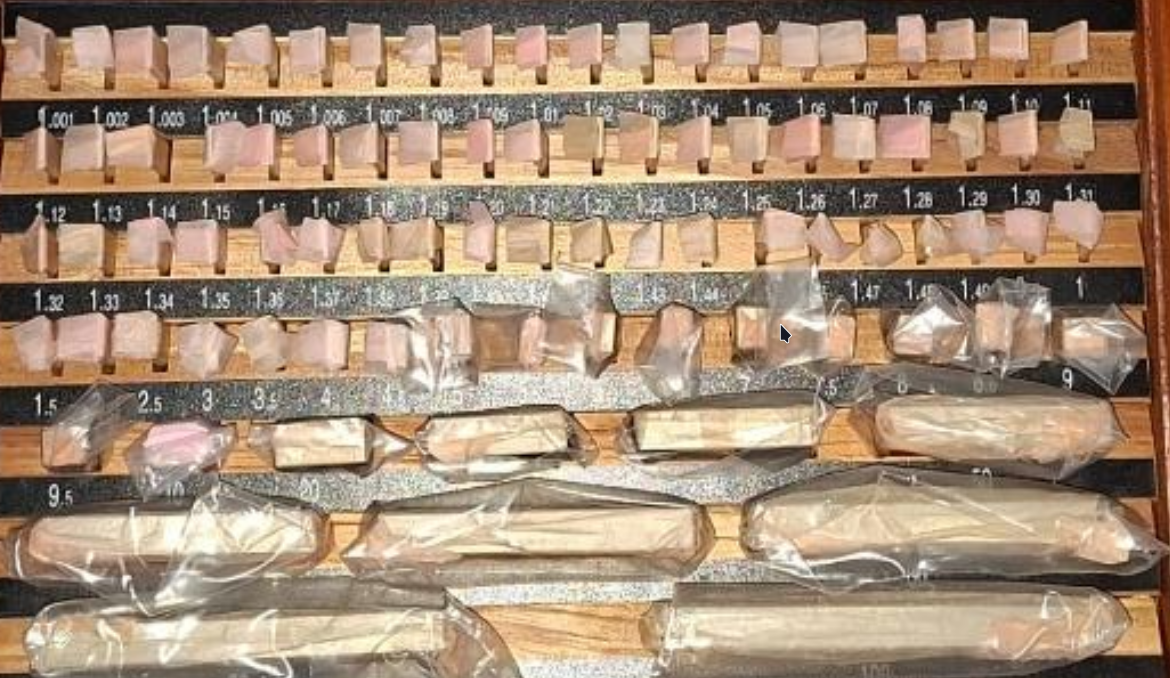
\includegraphics[width=0.55\textwidth]{img/patrones.png}
  \caption{Juego de bloques patrón de longitud.}
  \label{fig:bloques-instrumento}
\end{figure}

\subsubsection{Equipos de ensayos no destructivos para detección de fisuras}
\label{sec:instr-end}

\paragraph{Yugo electromagnético}
\label{sec:instr-yugo}

El yugo electromagnético es un equipo portátil de partículas magnéticas que
localiza discontinuidades superficiales y subsuperficiales en materiales
ferromagnéticos. Una bobina interna montada sobre un núcleo articulado con dos
patas ajustables induce un campo magnético local en la pieza; si una grieta
interrumpe las líneas de campo aparece una fuga de flujo magnético que atrae y
acumula las partículas aplicadas, revelando la falla. El fundamento físico se
desarrolla en la Sección~\ref{sec:mt}. El yugo Magnaflux Y-7 AC/DC tiene por
números de parte actuales 625643 (115~V) y 625644 (230~V); el número
43560 corresponde a una designación anterior del modelo de 230~V
\parencite{magnaflux_y7_yoke}. El modo de corriente alterna se usa para
defectos superficiales y el de corriente continua para fallas subsuperficiales,
conforme a ASTM E1444 e ISO 9934-1 \parencite{astm_e1444, iso9934_1}.

\begin{figure}[H]
  \centering
  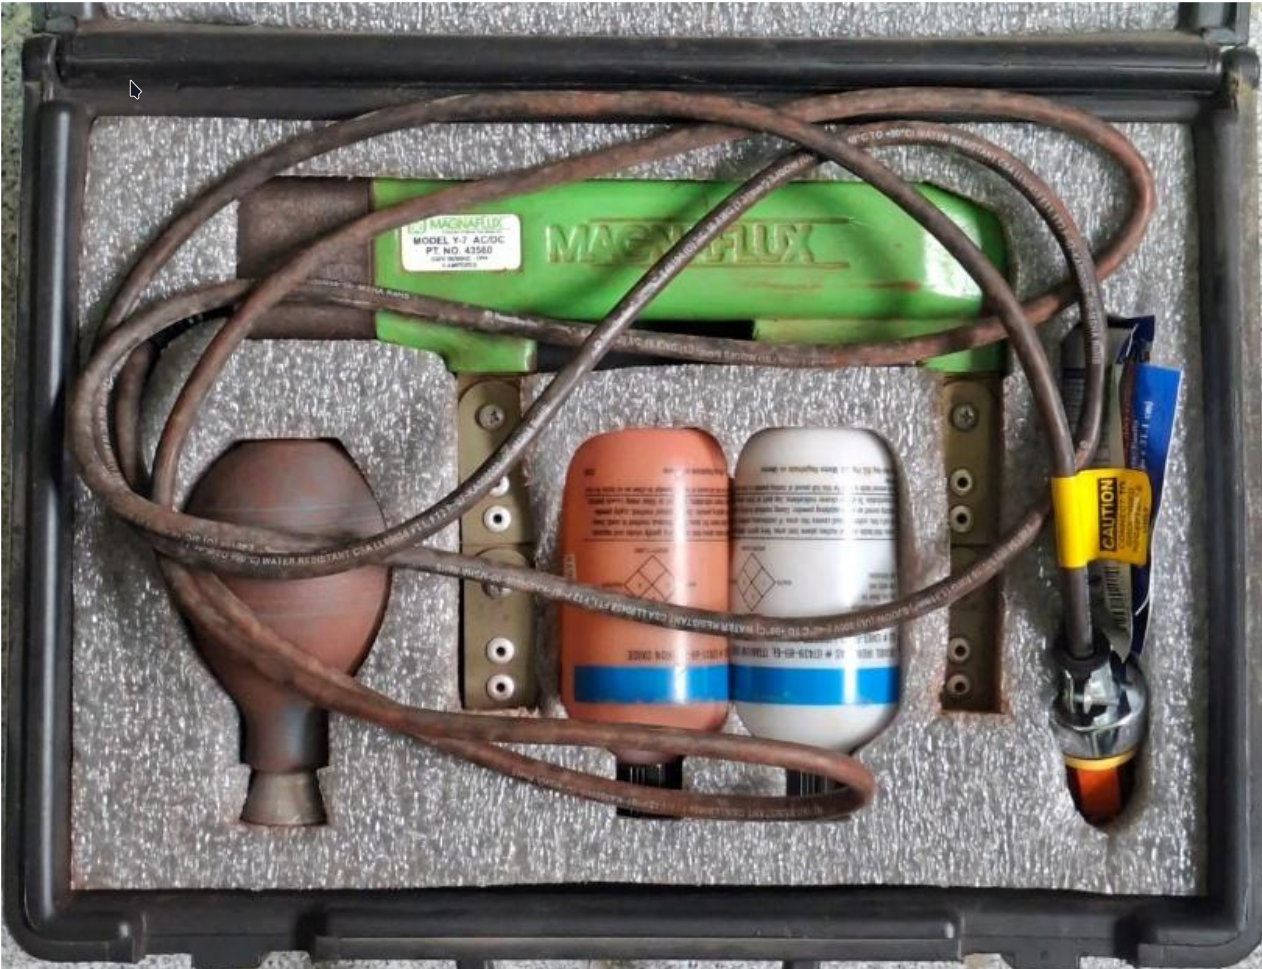
\includegraphics[width=0.45\textwidth]{img/yugo.png}
  \caption{Yugo Magnaflux Y-7 AC/DC (PT 43560) con sus accesorios.}
  \label{fig:yugo-instrumento}
\end{figure}

\paragraph{Lámpara de luz negra (radiación ultravioleta UV-A)}
\label{sec:instr-uv}

La lámpara de luz negra emite radiación UV-A en torno a $\lambda = 365\ \text{nm}$
y se emplea en los ensayos por líquidos penetrantes y partículas magnéticas
fluorescentes. Su función es excitar los pigmentos fotosensibles retenidos en
las fisuras para que emitan fluorescencia verde-amarilla, observable en
condiciones de oscuridad ambiental ($\le 20\ \text{lux}$). La irradiancia
requerida es de al menos $1000\ \mu\text{W/cm}^2$ a $38\ \text{cm}$ de distancia.
ASTM E3022 regula la medición de las características de emisión y los
requerimientos de las lámparas LED UV-A \parencite{astm_e3022_uv}, en tanto que
los criterios de irradiancia e iluminancia para la inspección se establecen en
ASTM E1417 y ASTM E1444 \parencite{astm_e1417, astm_e1444}. La secuencia
operativa se describe en las Secciones~\ref{sec:pt} y~\ref{sec:mt}.

\begin{figure}[H]
  \centering
  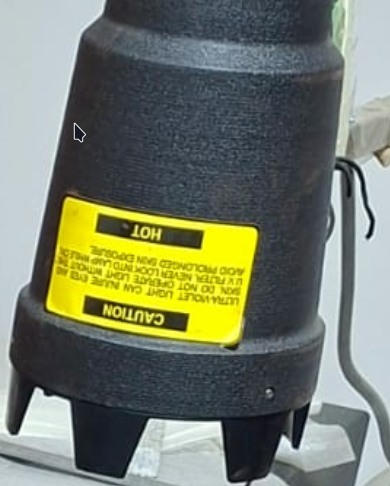
\includegraphics[width=0.30\textwidth]{img/lampara.png}
  \caption{Lámpara UV-A de inspección.}
  \label{fig:uv-instrumento}
\end{figure}


\subsection{Ensayos no destructivos}

\subsubsection{Inspección por líquidos penetrantes (PT)}
\label{sec:pt}

\paragraph{Fundamentos}

El ensayo por líquidos penetrantes es una técnica de ensayos no destructivos de
naturaleza fisicoquímica que permite detectar discontinuidades abiertas a la
superficie en materiales sólidos no porosos \parencite{astm_e165, hull1988}. El
penetrante moja la superficie y entra en la fisura por presión capilar
\parencite{kalinichenko2013}.

Para describir ese ingreso, tómese una fisura idealizada de ancho equivalente $R$ y
profundidad $h$. La ecuación de Rideal--Washburn \parencite{pmc_fluid_mech}
relaciona la profundidad alcanzada con el tiempo de permanencia:

\begin{equation}
  h^2(t) = \frac{\gamma \, R \, \cos\theta}{2\mu}\, t,
  \label{eq:rideal-washburn}
\end{equation}

donde $\gamma$ es la tensión superficial del líquido penetrante ($\text{N/m}$),
$\theta$ el ángulo de contacto dinámico entre el líquido y la pared de la fisura
($\cos\theta > 0$ para que haya mojabilidad), $\mu$ la viscosidad dinámica
($\text{Pa}\cdot\text{s}$) y $t$ el tiempo de permanencia o \textit{dwell time}.
De~\eqref{eq:rideal-washburn} se ve que $h$ crece con la raíz del tiempo: para
duplicar la profundidad hace falta cuadruplicar el tiempo de contacto, y un aumento
de $\mu$ o de $\theta$ frena la penetración. La
Figura~\ref{fig:pt-flujo-capilar} muestra el esquema de la fisura idealizada.

\begin{figure}[H]
  \centering
  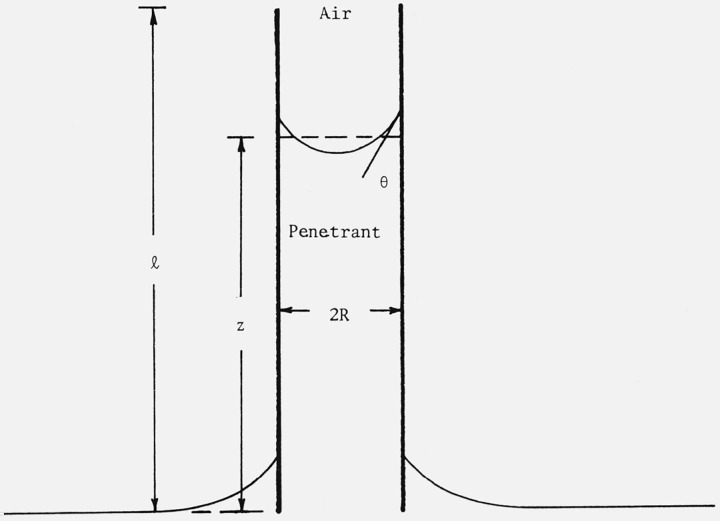
\includegraphics[width=0.55\textwidth]{figuras/deutsch-1979-flujo-capilar.jpg}
  \caption{Flujo capilar del penetrante en un tubo pequeño. Tomado de Deutsch
  (1979).}
  \label{fig:pt-flujo-capilar}
\end{figure}

Retirado el exceso de penetrante de la superficie, se aplica un medio poroso fino
llamado revelador. Éste se comporta como una esponja capilar inversa: absorbe el
líquido que quedó atrapado dentro de la fisura y forma una indicación visible cuyo
tamaño supera con creces el ancho real de la discontinuidad \parencite{almaguer2014}.
Por eso el método alcanza defectos muy por debajo de lo que distingue el ojo. La
Figura~\ref{fig:pt-falla} recoge una falla detectada de este modo en el espécimen 20
ensayado por Almaguer et al. (2014).

\begin{figure}[ht]
  \centering
  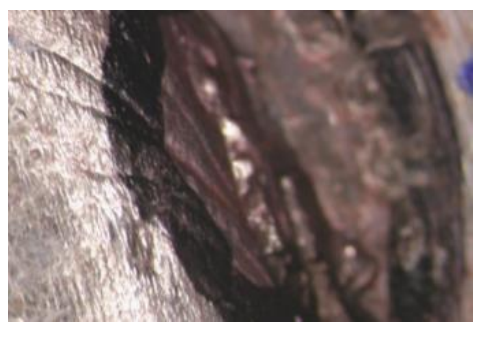
\includegraphics[width=0.42\textwidth]{figuras/almaguer-2014-falla-pt.png}
  \caption{Falla identificada por líquidos penetrantes en el espécimen 20. Adaptado
  de Almaguer et al. (2014).}
  \label{fig:pt-falla}
\end{figure}

\paragraph{Clasificación estandarizada del ensayo (ASTM E1417 / ISO 3452-1)}

De acuerdo con \parencite{astm_e1417, iso3452_1}, el proceso se clasifica según el
tipo de penetrante, el método de remoción del exceso y la forma del revelador.

\begin{enumerate}
  \item \textbf{Por tipo de penetrante:}
  \begin{itemize}
    \item \textbf{Tipo I (fluorescente):} contiene tintes fotosensibles que emiten
          fluorescencia verde-amarilla al excitarlos con radiación UV-A
          ($\lambda = 365\ \text{nm}$). Es el de mayor sensibilidad (niveles
          $1/2$ a $4$).
    \item \textbf{Tipo II (visible):} emplea colorantes rojos intensos que se
          observan con luz blanca natural o artificial ($\ge 1000\ \text{lux}$).
  \end{itemize}
  \item \textbf{Por método de remoción del exceso:}
  \begin{itemize}
    \item \textbf{lavable con agua}: el penetrante lleva agentes emulsionantes
          solubles en agua.
    \item \textbf{post-emulsionable lipofílico}: requiere aplicar después un
          emulsionante a base de aceite.
    \item \textbf{removible con solvente}: se elimina a mano con un paño impregnado
          en solvente no acuoso.
    \item \textbf{post-emulsionable hidrofílico}: usa un emulsionante diluido en agua
          antes del lavado final.
  \end{itemize}
  \item \textbf{Por forma de revelador:}
  \begin{itemize}
    \item polvo seco, aplicado en cámara de suspensión.
    \item soluble en agua.
    \item suspendible en agua.
    \item no acuoso para penetrante tipo I o II (aerosol con base de solvente).
  \end{itemize}
\end{enumerate}

\paragraph{Secuencia operativa estándar}

La inspección cuantitativa sigue seis etapas en orden \parencite{astm_e165}:

\begin{enumerate}
  \item \textbf{Limpieza previa.} Se quitan aceites, grasas, óxidos y pinturas
        mediante desengrase con solvente o ultrasonido.
  \item \textbf{Aplicación del penetrante y tiempo de morada.} Se aplica por
        inmersión, pulverización o pincel y se deja reposar entre $10$ y
        $30\ \text{min}$, según el material.
  \item \textbf{Remoción del exceso.} Se retira el penetrante de la superficie sin
        sacar el que quedó alojado dentro de los defectos.
  \item \textbf{Revelado.} Se extiende una capa delgada de revelador no acuoso
        (forma d) y se deja desarrollar al menos $10\ \text{min}$.
  \item \textbf{Inspección y evaluación.} Las indicaciones se interpretan en
        condiciones controladas: para el tipo II, con iluminación blanca
        $\ge 1000\ \text{lux}$; para el tipo I, con oscuridad ambiental
        ($\le 20\ \text{lux}$) e irradiancia UV-A
        $\ge 1000\ \mu\text{W/cm}^2$ a $38\ \text{cm}$ de distancia. La lámpara
        utilizada se describe en la Sección~\ref{sec:instr-uv}.
  \item \textbf{Limpieza posterior.} Se lava la pieza para evitar corrosión por
        residuos químicos.
\end{enumerate}

El método no detecta discontinuidades cerradas ni internas.

\subsubsection{Inspección por partículas magnéticas (MT)}
\label{sec:mt}

\paragraph{Fundamentos}

La inspección por partículas magnéticas es un END de tipo magnetoelectrostático que
sirve para localizar discontinuidades superficiales y subsuperficiales en materiales
de alta permeabilidad magnética ($\mu_r \gg 1$): aceros al carbono, aceros de baja
aleación y fundiciones ferromagnéticas \parencite{astm_e1444, lovejoy1993}.

El punto de partida es la segunda ecuación de Maxwell, $\nabla \cdot \vec{B} = 0$,
que descarta la existencia de monopolos magnéticos \parencite{rao2012}. Si se induce
un flujo $\Phi$ en una pieza ferromagnética mediante una fuerza magnetomotriz
$\mathcal{F} = N I$, la reluctancia del circuito sigue la ley de Hopkinson
\parencite{lovejoy1993}:

\begin{equation}
  \mathcal{F} = \Phi\,\mathcal{R},
  \qquad
  \mathcal{R} = \frac{l}{\mu_0\,\mu_r\,A},
  \label{eq:hopkinson-reluctancia}
\end{equation}

donde $l$ es la longitud del trayecto magnético, $A$ el área de la sección
transversal, $\mu_0 = 4\pi\times10^{-7}\ \text{H/m}$ la permeabilidad del vacío y
$\mu_r$ la permeabilidad relativa ($100 \le \mu_r \le 5000$).

Cuando el flujo cruza perpendicularmente una fisura de apertura $w$ llena de aire o
de contaminantes ($\mu_{aire}\approx 1$), la reluctancia local sube de golpe
($\mathcal{R}_{grieta} \gg \mathcal{R}_{mat}$). Ese gradiente obliga a las líneas de
campo a deformarse y a salir por la superficie, lo que produce un campo disperso
conocido como fuga de flujo magnético (\textit{Magnetic Flux Leakage}, MFL)
\parencite{rao2012}. Las partículas ferromagnéticas que se espolvorean encima son
atraídas hacia las zonas de mayor gradiente de $|\vec{B}|^2$ por la fuerza Kelvin:

\begin{equation}
  \vec{F}_m = \frac{V_p\,\chi_m}{\mu_0}\,\nabla |\vec{B}|^2,
  \label{eq:fuerza-kelvin}
\end{equation}

con $V_p$ el volumen de la partícula y $\chi_m$ su susceptibilidad magnética.

\begin{figure}[ht]
\centering
\begin{tikzpicture}[scale=0.9]
  % pieza ferromagnética
  \fill[gray!12] (0,0) rectangle (8,2);
  \draw[thick] (0,0) rectangle (8,2);

  % líneas de campo dentro de la pieza
  \foreach \y in {0.3,0.7,1.1,1.5,1.9} {
    \draw[-{Stealth}] (0.25,\y) -- (7.75,\y);
  }

  % grieta llena de aire
  \fill[white] (3.85,0.8) rectangle (4.15,2);
  \draw[thick] (3.85,2) -- (3.85,0.8) -- (4.15,0.8) -- (4.15,2);

  % fuga de flujo magnético
  \draw[-{Stealth}] (3.85,2) .. controls (3.35,2.9) and (4.65,2.9) .. (4.15,2);
  \draw[-{Stealth}] (3.85,2) .. controls (3.55,3.45) and (4.45,3.45) .. (4.15,2);

  % yugo
  \draw[very thick] (1.5,2) -- (1.5,3.6) -- (6.5,3.6) -- (6.5,2);

  % bobina sobre la barra superior
  \foreach \x in {3.0,3.3,...,5.0} {
    \draw[thick] (\x,3.6) -- (\x,3.95);
  }
  \draw[thick] (2.9,3.95) -- (5.1,3.95);

  % partículas magnéticas
  \foreach \p in {(3.6,2.1),(3.75,2.22),(4.25,2.24),(4.4,2.1),(3.5,2.02),(4.5,2.02)} {
    \fill \p circle (0.05);
  }

  % etiquetas
  \node[left] at (1.35,2.9) {yugo};
  \node at (4,4.15) {bobina};
  \node[right,fill=white,inner sep=1pt] at (4.3,0.95) {grieta};
  \node[right,font=\small] at (4.85,2.55) {partículas};
  \draw[-{Stealth},thin] (4.85,2.5) -- (4.55,2.2);
  \node[below] at (4,-0.1) {pieza ferromagnética};
\end{tikzpicture}
\caption{Esquema del ensayo por partículas magnéticas: el yugo magnetiza la pieza,
la grieta distorsiona el campo y las partículas se acumulan en la fuga de flujo.}
\label{fig:mt-esquema}
\end{figure}

\paragraph{Efecto piel y selección del tipo de corriente}

La profundidad con que el campo entra en el material depende de la frecuencia $f$ de
la corriente de magnetización, por el efecto piel. Esa profundidad se estima como
\parencite{rao2012}

\begin{equation}
  \delta = \sqrt{\frac{\rho}{\pi f \mu_0 \mu_r}},
  \label{eq:efecto-piel}
\end{equation}

donde $\rho$ es la resistividad del material ($\Omega\cdot\text{m}$).

\begin{itemize}
  \item \textbf{Corriente alterna (AC, $50/60\ \text{Hz}$).} Como $\delta \approx
        1\ \text{mm}$ en aceros, el campo se queda en la capa superficial y da la
        mayor sensibilidad para fisuras por fatiga abiertas a la superficie.
  \item \textbf{Corriente continua (DC) o rectificada de media onda (HWDC).} Al
        anular la frecuencia ($f\to 0$), el campo penetra en toda la sección y
        permite detectar fisuras subsuperficiales de hasta $3$ a $6\ \text{mm}$.
\end{itemize}

\paragraph{Clasificación estandarizada y métodos (ASTM E1444 / ISO 9934-1)}

Según \parencite{astm_e1444, iso9934_1, asme_bpvc_v}, las técnicas de magnetización
y los medios de detección se ordenan así:

\begin{enumerate}
  \item \textbf{Técnicas de inducción del campo:}
  \begin{itemize}
    \item \textbf{Magnetización longitudinal (yugo o bobina):} el campo va paralelo
          al eje del yugo o del solenoide y detecta grietas transversales a ese eje.
    \item \textbf{Magnetización circular (paso de corriente o conductor central):}
          la corriente circula por la pieza o por un conductor central y genera un
          campo anular, apto para fisuras longitudinales.
    \item \textbf{Magnetización multidireccional:} aplica campos cruzados en
          secuencias rápidas y cubre cualquier orientación en una sola operación.
  \end{itemize}
  \item \textbf{Medios de detección:}
  \begin{itemize}
    \item \textbf{Método seco:} partículas finas de hierro u óxidos coloreados
          (negro, rojo, amarillo) sopladas con aire; sirve para campo y piezas
          rugosas o soldaduras.
    \item \textbf{Método húmedo:} partículas en suspensión en aceite ligero o en
          agua con inhibidor de corrosión.
  \end{itemize}
  \item \textbf{Contraste y visualización:}
  \begin{itemize}
    \item \textbf{Visibles:} se inspeccionan con luz blanca intensa
          ($\ge 1000\ \text{lux}$).
    \item \textbf{Fluorescentes:} llevan pigmentos que emiten verde-amarillo bajo
          UV-A ($\lambda = 365\ \text{nm}$).
  \end{itemize}
\end{enumerate}

\paragraph{Verificación del yugo y secuencia operativa}

El yugo empleado se describe en la Sección~\ref{sec:instr-yugo}. La validez del
ensayo exige comprobar periódicamente su fuerza (\textit{Yoke Lift Test})
conforme a ASTM E1444 \parencite{astm_e1444}:

\begin{itemize}
  \item \textbf{Yugo de AC:} debe levantar una placa patrón de acero de al menos
        $4.5\ \text{kg}$ ($10\ \text{lb}$) con la separación de polos de trabajo.
  \item \textbf{Yugo de DC:} debe levantar al menos $18.1\ \text{kg}$
        ($40\ \text{lb}$).
\end{itemize}

La secuencia estándar tiene estas fases \parencite{iso9934_1}:

\begin{enumerate}
  \item \textbf{Preparación de la superficie.} Se limpian grasa, escamas de
        laminación, pintura suelta y residuos magnéticos.
  \item \textbf{Posicionamiento del yugo y magnetización.} Los polos se apoyan
        perpendiculares a la dirección esperada de la grieta.
  \item \textbf{Aplicación continua de partículas.} El medio húmedo o seco se
        dispersa mientras la corriente sigue activa (\textit{método continuo}).
  \item \textbf{Inspección visual y evaluación.} Con partículas visibles se requiere
        $\ge 1000\ \text{lux}$; con fluorescentes, oscuridad ambiental
        $\le 20\ \text{lux}$ e irradiancia UV-A
        $\ge 1000\ \mu\text{W/cm}^2$ a $38\ \text{cm}$.
  \item \textbf{Desmagnetización residual.} Se aplica un campo alterno decreciente e
        invertido para bajar la inducción remanente de $0.3\ \text{mT}$
        ($3\ \text{Gauss}$) \parencite{astm_e1444}.
\end{enumerate}

El yugo solo es aplicable a materiales ferromagnéticos y exige desmagnetización
posterior \parencite{astm_e1444}.

\subsubsection{Inspección por ultrasonido (UT) y medición de espesores}
\label{sec:ut}

\paragraph{Fundamentos}

La inspección por ultrasonido es un método volumétrico de END que se apoya en la
propagación de ondas elásticas de alta frecuencia ($0.5$ a $25\ \text{MHz}$) por
medios sólidos homogéneos \parencite{krautkramer1990, iso16810}.

En un sólido elástico e isótropo, la velocidad de una onda longitudinal $c_L$ depende
del módulo de Young $E$, del coeficiente de Poisson $\nu$ y de la densidad $\rho$
\parencite{cheeke2017}:

\begin{equation}
  c_L = \sqrt{\frac{E(1-\nu)}{\rho(1+\nu)(1-2\nu)}}.
  \label{eq:velocidad-longitudinal}
\end{equation}

Para el acero al carbono a $20\ ^\circ\text{C}$ se tiene $c_L \approx
5920\ \text{m/s}$.

La medición de espesores por eco de pulso (\textit{pulse-echo}) consiste en medir el
tiempo de vuelo de ida y vuelta, $\Delta t$, que tarda el pulso en ir de la superficie
de entrada a la pared posterior (o a una discontinuidad) y volver al receptor
\parencite{astm_e797}:

\begin{equation}
  e = \frac{c_L\,\Delta t}{2}.
  \label{eq:espesor-tof}
\end{equation}

Al llegar a la interfaz entre el material ($Z_1$) y el medio exterior o la grieta
($Z_2$), la onda se refleja y se refracta según la diferencia de impedancia acústica
$Z = \rho c_L$ ($\text{Pa}\cdot\text{s/m}$). El coeficiente de reflexión en
intensidad, en incidencia normal, es \parencite{krautkramer1990}

\begin{equation}
  R = \left(\frac{Z_2 - Z_1}{Z_2 + Z_1}\right)^2.
  \label{eq:coeficiente-reflexion}
\end{equation}

En la interfaz acero-aire ($Z_{acero}\approx 45\times10^6\ \text{Pa}\cdot\text{s/m}$
frente a $Z_{aire}\approx 400\ \text{Pa}\cdot\text{s/m}$), $R\approx 0.9999$: casi
toda la energía ($99.99\%$) vuelve, lo que permite detectar grietas y medir
espesores con buena resolución.

\paragraph{Acoplamiento acústico y transductores piezoeléctricos}

El pulso se genera y se recibe por efecto piezoeléctrico inverso y directo en
cristales sintéticos de titanato zirconato de plomo (PZT) o niobato de litio
\parencite{cheeke2017}.

\begin{itemize}
  \item \textbf{Transductores de elemento dual.} Llevan dos cristales independientes
        sobre suelas en ángulo, uno emisor y otro receptor, separados por una barrera
        de aislamiento acústico. Así se elimina el ruido de campo cercano y la zona
        muerta, lo que mejora la medición de espesores delgados
        ($0.8$ a $50\ \text{mm}$) y la detección de corrosión interna (picaduras)
        \parencite{astm_e797}.
  \item \textbf{Acoplante acústico.} Como el aire en la interfaz sonda-pieza bloquea
        la onda ($R\to 1$), se aplica un fluido o gel (glicerina, gel acuoso o aceite
        mineral) que elimina la película de aire y deja pasar el pulso.
\end{itemize}

\paragraph{Procedimiento de calibración según INACAL PC-029}

La calibración de un medidor digital de espesores por ultrasonido, descrito en la
Sección~\ref{sec:instr-ut}, sigue el procedimiento INACAL PC-029
\parencite{inacal_pc029, astm_e797}:

\begin{enumerate}
  \item \textbf{Ajuste del cero del palpador.} Se compensa el retardo acústico que
        introduce la suela del transductor.
  \item \textbf{Ajuste de la velocidad del sonido.} El instrumento se calibra con un
        bloque patrón de acero a dos espesores acotados, por ejemplo
        $L_1 = 2.5\ \text{mm}$ y $L_2 = 20.0\ \text{mm}$.
  \item \textbf{Verificación de linealidad.} Se evalúan cinco puntos uniformes de un
        bloque patrón escalonado (\textit{step block}) con trazabilidad nacional o
        internacional.
  \item \textbf{Incertidumbre combinada.} Conforme a la guía GUM
        \parencite{jcgm2008gum}, la incertidumbre del espesor medido se compone de
        \begin{equation}
          u_c^2(d) = u^2(\bar{d}_{rep}) + u^2(d_{res}) + u^2(L_{BP})
                     + u^2(\delta c_L) + u^2(\delta T),
          \label{eq:ut-incertidumbre}
        \end{equation}
        donde $u(\bar{d}_{rep}) = s/\sqrt{n}$ es la repetibilidad (tipo A),
        $u(d_{res}) = d_{res}/(2\sqrt{3})$ la resolución del display y
        $u(\delta c_L)$ recoge la variabilidad del material.
\end{enumerate}

\paragraph{Modos de presentación de datos ultrasónicos}

La Figura~\ref{fig:ut-modos} resume los tres modos con que se presenta la señal.

\begin{figure}[ht]
\centering
\begin{tikzpicture}[scale=0.82]
  % (a) A-Scan
  \begin{scope}
    \draw[-{Stealth}] (0,0) -- (4.2,0) node[right,font=\scriptsize] {$t$};
    \draw[-{Stealth}] (0,0) -- (0,2.2) node[above,font=\scriptsize] {$A$};
    \draw[thick] (0.15,0.1) -- (3.9,0.1);
    \draw[thick] (0.35,0.1) -- (0.45,1.55) -- (0.55,0.1);
    \draw[thick] (0.65,0.1) -- (0.8,0.28) -- (0.95,0.08)
                 -- (1.1,0.24) -- (1.25,0.07) -- (1.4,0.2)
                 -- (1.55,0.06) -- (1.7,0.16) -- (1.85,0.05)
                 -- (2.0,0.13) -- (2.15,0.04) -- (2.3,0.1) -- (2.45,0.05);
    \draw[thick] (2.65,0.05) -- (2.75,1.15) -- (2.85,0.05);
    \node[font=\scriptsize] at (2.1,-0.55) {(a) A-Scan};
  \end{scope}

  % (b) B-Scan
  \begin{scope}[shift={(5.3,0)}]
    \fill[gray!12] (0,0) rectangle (4,2);
    \draw (0,0) rectangle (4,2);
    \fill[gray!55] (0,1.55) rectangle (4,1.75);
    \fill[black!80] (2.1,0.55) rectangle (2.45,0.85);
    \draw[-{Stealth}] (0,-0.15) -- (4.2,-0.15) node[right,font=\scriptsize] {$x$};
    \draw[-{Stealth}] (-0.15,0) -- (-0.15,2.15) node[above,font=\scriptsize] {$t$};
    \node[font=\scriptsize] at (2.1,-0.55) {(b) B-Scan};
  \end{scope}

  % (c) C-Scan
  \begin{scope}[shift={(10.6,0)}]
    \fill[gray!10] (0,0) rectangle (4,2);
    \draw (0,0) rectangle (4,2);
    \fill[red!20] (2.0,0.9) circle (0.55);
    \fill[red!60] (2.0,0.9) circle (0.3);
    \draw[-{Stealth}] (0,-0.15) -- (4.2,-0.15) node[right,font=\scriptsize] {$x$};
    \draw[-{Stealth}] (-0.15,0) -- (-0.15,2.15) node[above,font=\scriptsize] {$y$};
    \node[font=\scriptsize] at (2.1,-0.55) {(c) C-Scan};
  \end{scope}
\end{tikzpicture}
\caption{Modos de presentación de datos ultrasónicos: (a) A-Scan, amplitud frente al
tiempo de vuelo; (b) B-Scan, corte transversal con la indicación del defecto;
(c) C-Scan, vista en planta con la posición del reflector.}
\label{fig:ut-modos}
\end{figure}

\begin{itemize}
  \item \textbf{A-Scan (amplitud).} Gráfica unidimensional de la señal RF o
        rectificada: la amplitud del eco ($y$) frente al tiempo de vuelo o la
        distancia ($x$).
  \item \textbf{B-Scan (corte transversal).} Representación bidimensional del perfil
        de la pieza a lo largo de una línea de escaneo; sirve para ver mapas de
        corrosión y pérdida de pared.
  \item \textbf{C-Scan (vista de planta).} Mapeo en el plano $x$-$y$ que muestra la
        profundidad o la amplitud de los reflectores en toda el área inspeccionada.
\end{itemize}

\subsubsection{Inspección visual (VT)}
\label{sec:vt}

\paragraph{Fundamentos}

La inspección visual es el método primario de los END: se realiza antes que cualquier
otra técnica, superficial o volumétrica, y no necesita equipos especiales
\parencite{asme_bpvc_v_art9, iso17637}. Se apoya en la interacción de la luz visible
($\lambda \in [380,780]\ \text{nm}$) con la superficie de la pieza y en la respuesta
del ojo o de un sensor electroóptico \parencite{moore2012}.

La iluminación que llega al inspector sigue la ley del inverso del cuadrado de la
distancia y el teorema del coseno de Lambert \parencite{cheeke2017}:

\begin{equation}
  E_v = \frac{I_v \cos\theta}{r^2},
  \label{eq:iluminancia-lambert}
\end{equation}

donde $E_v$ es la iluminancia sobre la superficie ($\text{lux} = \text{lm/m}^2$),
$I_v$ la intensidad luminosa de la fuente (candela), $r$ la distancia de la fuente al
punto de inspección (m) y $\theta$ el ángulo entre la luz y la normal a la superficie.

La resolución espacial del ojo, $\Delta x_{min}$, se deduce del umbral de agudeza
visual angular $\theta_{min}\approx 1$ minuto de arco $= 2.91\times10^{-4}\ \text{rad}$
\parencite{moore2012}:

\begin{equation}
  \Delta x_{min} = d_{vis}\tan\theta_{min} \approx d_{vis}\,\theta_{min}.
  \label{eq:agudeza-visual}
\end{equation}

A la distancia de visión cercana, $d_{vis} = 250\ \text{mm}$, queda
$\Delta x_{min}\approx 0.07\ \text{mm}$ ($70\ \mu\text{m}$).

\paragraph{Clasificación estandarizada del ensayo (ISO 17637 / ASME Sec. V Art. 9)}

Conforme a \parencite{asme_bpvc_v_art9, iso17637}, la técnica se divide según la
accesibilidad de la pieza:

\begin{enumerate}
  \item \textbf{Inspección visual directa.} Se usa cuando hay línea de visión directa
        e ininterrumpida. Para asegurar la confiabilidad, las normas fijan la
        geometría de observación \parencite{iso17637}:
  \begin{itemize}
    \item \textbf{Distancia de visión:} el ojo no debe estar a más de
          $600\ \text{mm}$ ($24\ \text{pulg}$) de la superficie.
    \item \textbf{Ángulo de visión:} el ángulo entre la línea de visión y el plano de
          la superficie no debe ser menor de $30^\circ$.
    \item \textbf{Instrumentación auxiliar:} lupas de $2\times$ a $10\times$, espejos
          planos articulados, linternas LED de alta intensidad y galgas de soldadura
          (Cambridge, Hi-Lo, escala de filete y micrómetros de profundidad).
  \end{itemize}
  \item \textbf{Inspección visual remota o indirecta (RVT).} Se emplea en cavidades
        internas, tuberías de diámetro reducido, recipientes a presión o zonas de
        alta radiación donde no se puede acceder \parencite{asme_bpvc_v_art9}.
        Usa sistemas ópticos y optoelectrónicos:
  \begin{itemize}
    \item \textbf{Boroscopios rígidos:} lentes acromáticas en tubo metálico con guía
          de luz de fibra óptica; buena resolución angular, pero ángulo de visión
          fijo.
    \item \textbf{Fibroscopios flexibles:} haz de fibras ópticas coherentes para la
          imagen y fibras desordenadas para la iluminación.
    \item \textbf{Videoendoscopios digitales:} cabezales articulados con sensor
          CCD/CMOS en la punta, iluminación LED y procesamiento digital, con
          medición tridimensional por estereofotogrametría o escaneo láser
          \parencite{moore2012}.
  \end{itemize}
\end{enumerate}

\begin{figure}[ht]
\centering
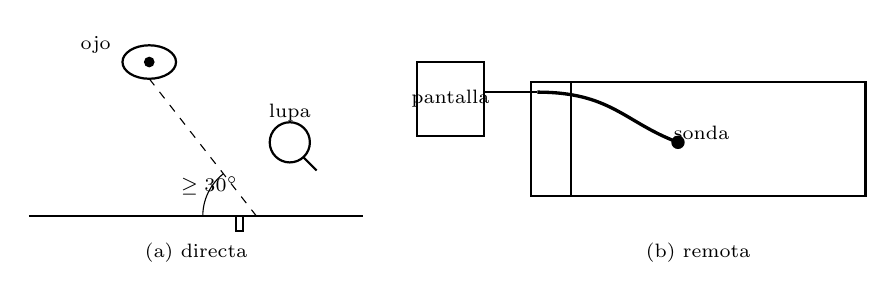
\begin{tikzpicture}[scale=0.85]
  % (a) inspección directa
  \begin{scope}
    \draw[thick] (0,0) -- (5,0);
    \draw[thick] (1.8,2.3) ellipse (0.4 and 0.25);
    \fill (1.8,2.3) circle (0.08);
    \draw[dashed] (1.8,2.05) -- (3.4,0);
    \draw (2.6,0) arc (180:128:0.8);
    \node[font=\scriptsize] at (2.7,0.45) {$\ge 30^\circ$};
    \node[font=\scriptsize] at (1.0,2.55) {ojo};
    % lupa
    \draw[thick] (3.9,1.1) circle (0.3);
    \draw[thick] (4.1,0.88) -- (4.3,0.68);
    \node[font=\scriptsize] at (3.9,1.55) {lupa};
    % defecto superficial
    \draw[thick] (3.1,0) -- (3.1,-0.22) -- (3.2,-0.22) -- (3.2,0);
    \node[font=\scriptsize] at (2.5,-0.55) {(a) directa};
  \end{scope}

  % (b) inspección remota
  \begin{scope}[shift={(7.5,0)}]
    \draw[thick] (0,0.3) -- (5,0.3) -- (5,2) -- (0,2) -- cycle;
    \draw[thick] (0.6,0.3) -- (0.6,2);
    \draw[very thick] (0.1,1.85) .. controls (1.2,1.85) and (1.4,1.4) .. (2.2,1.1);
    \fill (2.2,1.1) circle (0.1);
    \node[font=\scriptsize] at (2.55,1.25) {sonda};
    % cable y pantalla
    \draw[thick] (0.1,1.85) -- (-0.7,1.85);
    \draw[thick] (-1.7,1.2) rectangle (-0.7,2.3);
    \node[font=\scriptsize] at (-1.2,1.75) {pantalla};
    \node[font=\scriptsize] at (2.5,-0.55) {(b) remota};
  \end{scope}
\end{tikzpicture}
\caption{Inspección visual: (a) directa, con la línea de visión y el ángulo mínimo de
observación; (b) remota, con una sonda videoendoscópica en el interior de una
cavidad.}
\label{fig:vt-directa-remota}
\end{figure}

\paragraph{Secuencia operativa en uniones soldadas}

En uniones soldadas de acero estructural o tuberías, la inspección visual se hace en
tres fases \parencite{iso17637}:

\begin{enumerate}
  \item \textbf{Antes del soldeo.} Se verifica el ángulo de bisel, la apertura de
        raíz (\textit{root gap}), la alineación de bordes (\textit{hi-lo}), la
        ausencia de óxido, pintura o humedad y la conformidad de los materiales de
        aporte.
  \item \textbf{Durante el soldeo.} Se revisa la pasada de raíz, la limpieza de
        escoria entre pases y la posible aparición de grietas de solidificación o
        poros.
  \item \textbf{Después del soldeo.} Se evalúan la forma y el sobreespesor del
        refuerzo, las socavaciones (\textit{undercut}), la falta de llenado
        (\textit{underfill}), los traslapes (\textit{overlap}), las porosidades
        abiertas, las salpicaduras (\textit{spatter}) y el socavamiento de raíz.
\end{enumerate}

\paragraph{Requisitos ambientales y calificación del personal}

\begin{itemize}
  \item \textbf{Iluminancia.} ISO 17637 exige al menos $350\ \text{lux}$ sobre la
        superficie para inspección general y recomienda $1000\ \text{lux}$ para
        caracterizar microfisuras \parencite{iso17637}.
  \item \textbf{Calificación del inspector.} Debe acreditar cada año agudeza visual
        cercana con la carta Jaeger N.º 1 (o el equivalente ISO 18490 a
        $30\ \text{cm}$) y distinguir contrastes cromáticos (test de Ishihara),
        conforme a ISO 9712 o ASNT SNT-TC-1A \parencite{iso9712}.
\end{itemize}


